\chapter{Fine Tune A Pre-Trained Model}
L'obiettivo di questa parte è stato quello di cercare di ottenere le migliori performance possibili da una CNN su un dataset diverso da quello su cui la rete è stata pre-addestrata.

È stata prima stabilita una baseline con un classico classificatore standard.

\subsection{Scelte}
Fino a questo momento l'obiettivo non era basato sulle prestazioni; come abbiamo già spiegato nei Capitoli \ref{chap:MLP} e \ref{chap:CNN} l'architettura delle reti usate è stata definita senza un qualche razionale che incrementasse una qualche metrica, ma solo per dimostrare che la profondità non è direttamente proporzionale alle prestazioni. Per questo motivo non ho preso una delle reti definite in precedenza, ma ho usato un modello noto, già definito e strutturato per massimizzare le prestazioni: ResNet-18.

\myskip

Il dataset scelto per eseguire gli esperimenti è CIFAR-100. Come già analizzato nella Sezione \ref{sec:CIFAR100}, questo è più complesso per quanto riguarda tipo e specializzazione delle classi, e quindi rende più complesso il compito. Visto l'obiettivo si è deciso di usare un validation set: il train set di partenza, composto da 50K elementi, è stato suddiviso in un train set di 45K elementi e un validation set di 5K.

Durante i vari cicli di addestramento il test set è stato dimenticato (come se non ci fosse). Solo alla fine è stato poi utilizzato per vedere come i migliori modelli generalizzano su dati mai visti.

%%%%%%%%%%%%%%%%%%%%%%%%%%%%%%%%%%%%%%%%%%%%%%%%%%%%
\section{Baseline}
Per stabilire una baseline su CIFAR-100 sono state valutate le performance di due modelli di classificazione classici: SVM e Logistic Regression.

\myskip

L'addestramento di questi due classificatori è stato fatto sulle features estratte da ResNet-18 su CIFAR-100. I pesi di ResNet sono ricavati dall'addestramento su CIFAR-10. Per l'estrazione di features è stato fondamentale rimuovere l'ultimo layer lineare presente in ResNet; in questo modo le features estratte sono il risultato dell'ultimo average pooling della rete.

Per l'addestramento della ResNet è stato necessario sostituire l'ultimo layer lineare, che ha dimensionalità dell'output 1000, con uno che avesse una dimensione in uscita di 10 classi (le 10 classi di CIFAR-10). Con questo approccio l'accuracy ottenuta dai due classificatori è stata di circa 0,37.

%%%%%%%%%%%%%%%%%%%%%%%%%%%%%%%%%%%%%%%%%%%%%%%%%%%%
\section{Fine tune}
\label{sec:finetune}
Come primo tentativo per aumentare le performance ho cercato di fare fine tuning del modello addestrato su CIFAR-10. Per prima cosa, prima di procedere all'addestramento su CIFAR-100, ho dovuto modificare l'ultimo layer lineare, quello che si occupa della classificazione, in modo che la dimensione dell'output sia 100 e non 10.

\myskip

Ho provato a congelare i pesi di tutti i layer tranne quelli del nuovo layer lineare (\texttt{nn.Linear()}), in quello che è stato definito l'esperimento fine\_tune\_1; in questo modo tutti i pesi restano gli stessi, tranne quelli che sono responsabili della classificazione vera e propria. Con questa soluzione l'accuracy registrata è stata inferiore alla baseline, con un valore di circa 0,29.

Successivamente ho scongelato i pesi del quarto layer. In un primo momento l'idea era quella di abbassare il valore della loss, portandola da $5\cdot10^{-4}$ a $10^{-5}$. Osservando però le curve della loss sul train set e dell'accuracy dell'addestramento precedente, si può notare come non siamo ancora arrivati ad un asintoto, per cui ho deciso di lasciarlo invariato.
Come si mostra però dalla Figura \ref{fig:finetune1}, questo approccio ha portato ad avere overfitting; si nota infatti che la loss sul train set è praticamente a 0.

\begin{figure}[htbp]
    \centering
    \begin{subfigure}{0.45\textwidth}
        \centering
        \includegraphics[width=\textwidth]{immages/5-fine tune/loss finetune 1.pdf}
        \caption{Loss}
    \end{subfigure}
    \hfill
    \begin{subfigure}{0.45\textwidth}
        \centering
        \includegraphics[width=\textwidth]{immages/5-fine tune/acc finetune 1.pdf}
        \caption{Accuracy}
    \end{subfigure}
    \caption{Fine tune con stesso learning rate.}
    \label{fig:finetune1}
\end{figure}

\myskip

Per cercare di mitigare il problema ho abbassato il learning rate quando ho addestrato i layer precedenti all'ultimo (esperimenti fine\_tune\_x\_lr), ma con un learning rate di un ordine inferiore. I risultati, mostrati in Figura \ref{fig:finetune2}, sono stati più soddisfacenti: la loss ha una discesa molto più regolare; l'accuracy ha raggiunto i livelli di quella dell'esperimento fine\_tune\_2 ma probabilmente la generalizzazione è migliore. L'ultima osservazione che si può fare è sui valori alti della loss: si può notare che la curva di discesa (così come quella di salita dell'accuracy) non ha raggiunto un asintoto; molto probabilmente con più epoche il modello si adatterebbe meglio ai dati e avremmo risultati migliori.

\begin{figure}[htbp]
    \centering
    \begin{subfigure}{0.45\textwidth}
        \centering
        \includegraphics[width=\textwidth]{immages/5-fine tune/loss finetune 2.pdf}
        \caption{Loss}
    \end{subfigure}
    \hfill
    \begin{subfigure}{0.45\textwidth}
        \centering
        \includegraphics[width=\textwidth]{immages/5-fine tune/acc finetune 2.pdf}
        \caption{Accuracy}
    \end{subfigure}
    \caption{Fine tune con learning rate decrescente}
    \label{fig:finetune2}
\end{figure}

\myskip

Non ho scongelato altri layer perché altrimenti ci saremmo allontanati dal nostro obiettivo. Se scongelassimo tutti i layer non staremmo facendo altro che un classico addestramento di ResNet su CIFAR-100 a partire da pesi non inizializzati casualmente; quello che vogliamo invece è ottimizzare le prestazioni di un modello già addestrato.

%%%%%%%%%%%%%%%%%%%%%%%%%%%%%%%%%%%%%%%%%%%%%%%%%%%%
\section{Early stopping}
Nel seguito continuiamo ad addestrare il modello di ResNet variando solo i pesi degli ultimi due layer più quello di classificazione. Manteniamo quindi congelati i pesi dei primi layer della rete.

\myskip

Per cercare di migliorare la generalizzazione del modello ho applicato la tecnica di early stopping. L'idea è quella di monitorare l'accuracy sul validation set e di interrompere l'addestramento se non migliora di una data tolleranza per un certo numero di epoche (la "patience").

Per vedere l'early stopping in azione senza utilizzare moltissime epoche e non avere tempi di addestramento lunghissimi (in pratica solo per avere un esperimento fittizio), ho dovuto tenere un learning rate alto ($5\cdot10^{-3}$) e una patience bassa (5).
Osservando la Figura \ref{fig:earlystopping} si può notare esattamente questo: la loss sul train set raggiunge un valore molto basso; l'accuracy inizia a oscillare senza però migliorare.

\myskip

Questo è un esempio fittizio e probabilmente poco utile, ma sicuramente fa capire quanto questa tecnica possa diventare utile per fermare l'addestramento sotto determinate condizioni.

\begin{figure}[htbp]
    \centering
    \begin{subfigure}{0.45\textwidth}
        \centering
        \includegraphics[width=\textwidth]{immages/5-fine tune/loss es.pdf}
        \caption{Loss}
    \end{subfigure}
    \hfill
    \begin{subfigure}{0.45\textwidth}
        \centering
        \includegraphics[width=\textwidth]{immages/5-fine tune/acc es.pdf}
        \caption{Accuracy}
    \end{subfigure}
    \caption{Esperimento con early stopping con \texttt{patience=5}}
    \label{fig:earlystopping}
\end{figure}
%%%%%%%%%%%%%%%%%%%%%%%%%%%%%%%%%%%%%%%%%%%%%%%%%%%%
\section{Optimizer}
Ho cercato di variare l'algoritmo di ottimizzazione per cercare di capire quale si adattasse al problema. In tutti gli addestramenti è stata usata la tecnica di early stopping implementata in precedenza. Gli ottimizzatori testati sono stati:
\begin{itemize}
    \item Adam
    \item SGD
    \item AdamW, che migliora la generalizzazione del modello con la tecnica weight decay.
    \item RMSprop, che migliora SGD con la scelta del learning rate dinamicamente basandosi su una media dei gradienti.
\end{itemize}

Un primo approccio è stato quello di usare un learning rate di $5\cdot10^{-4}$, ma non ha funzionato bene. Come si può vedere dalla Figura \ref{fig:opt1} tutte le funzioni di ottimizzazione sono state soggette ad overfitting, tranne SGD che è anche l'unico che ha attivato l'early stopping (ma ha comunque avuto prestazioni non soddisfacenti).

Questo risultato ha evidenziato quanto già avevamo capito dalla prima parte della Sezione \ref{sec:finetune}: quando si scongelano solo alcuni layer conviene procedere più lentamente, tramite un learning rate basso, per avvicinarsi in modo più preciso alla soluzione.

\begin{figure}[htbp]
    \centering
    \begin{subfigure}{0.45\textwidth}
        \centering
        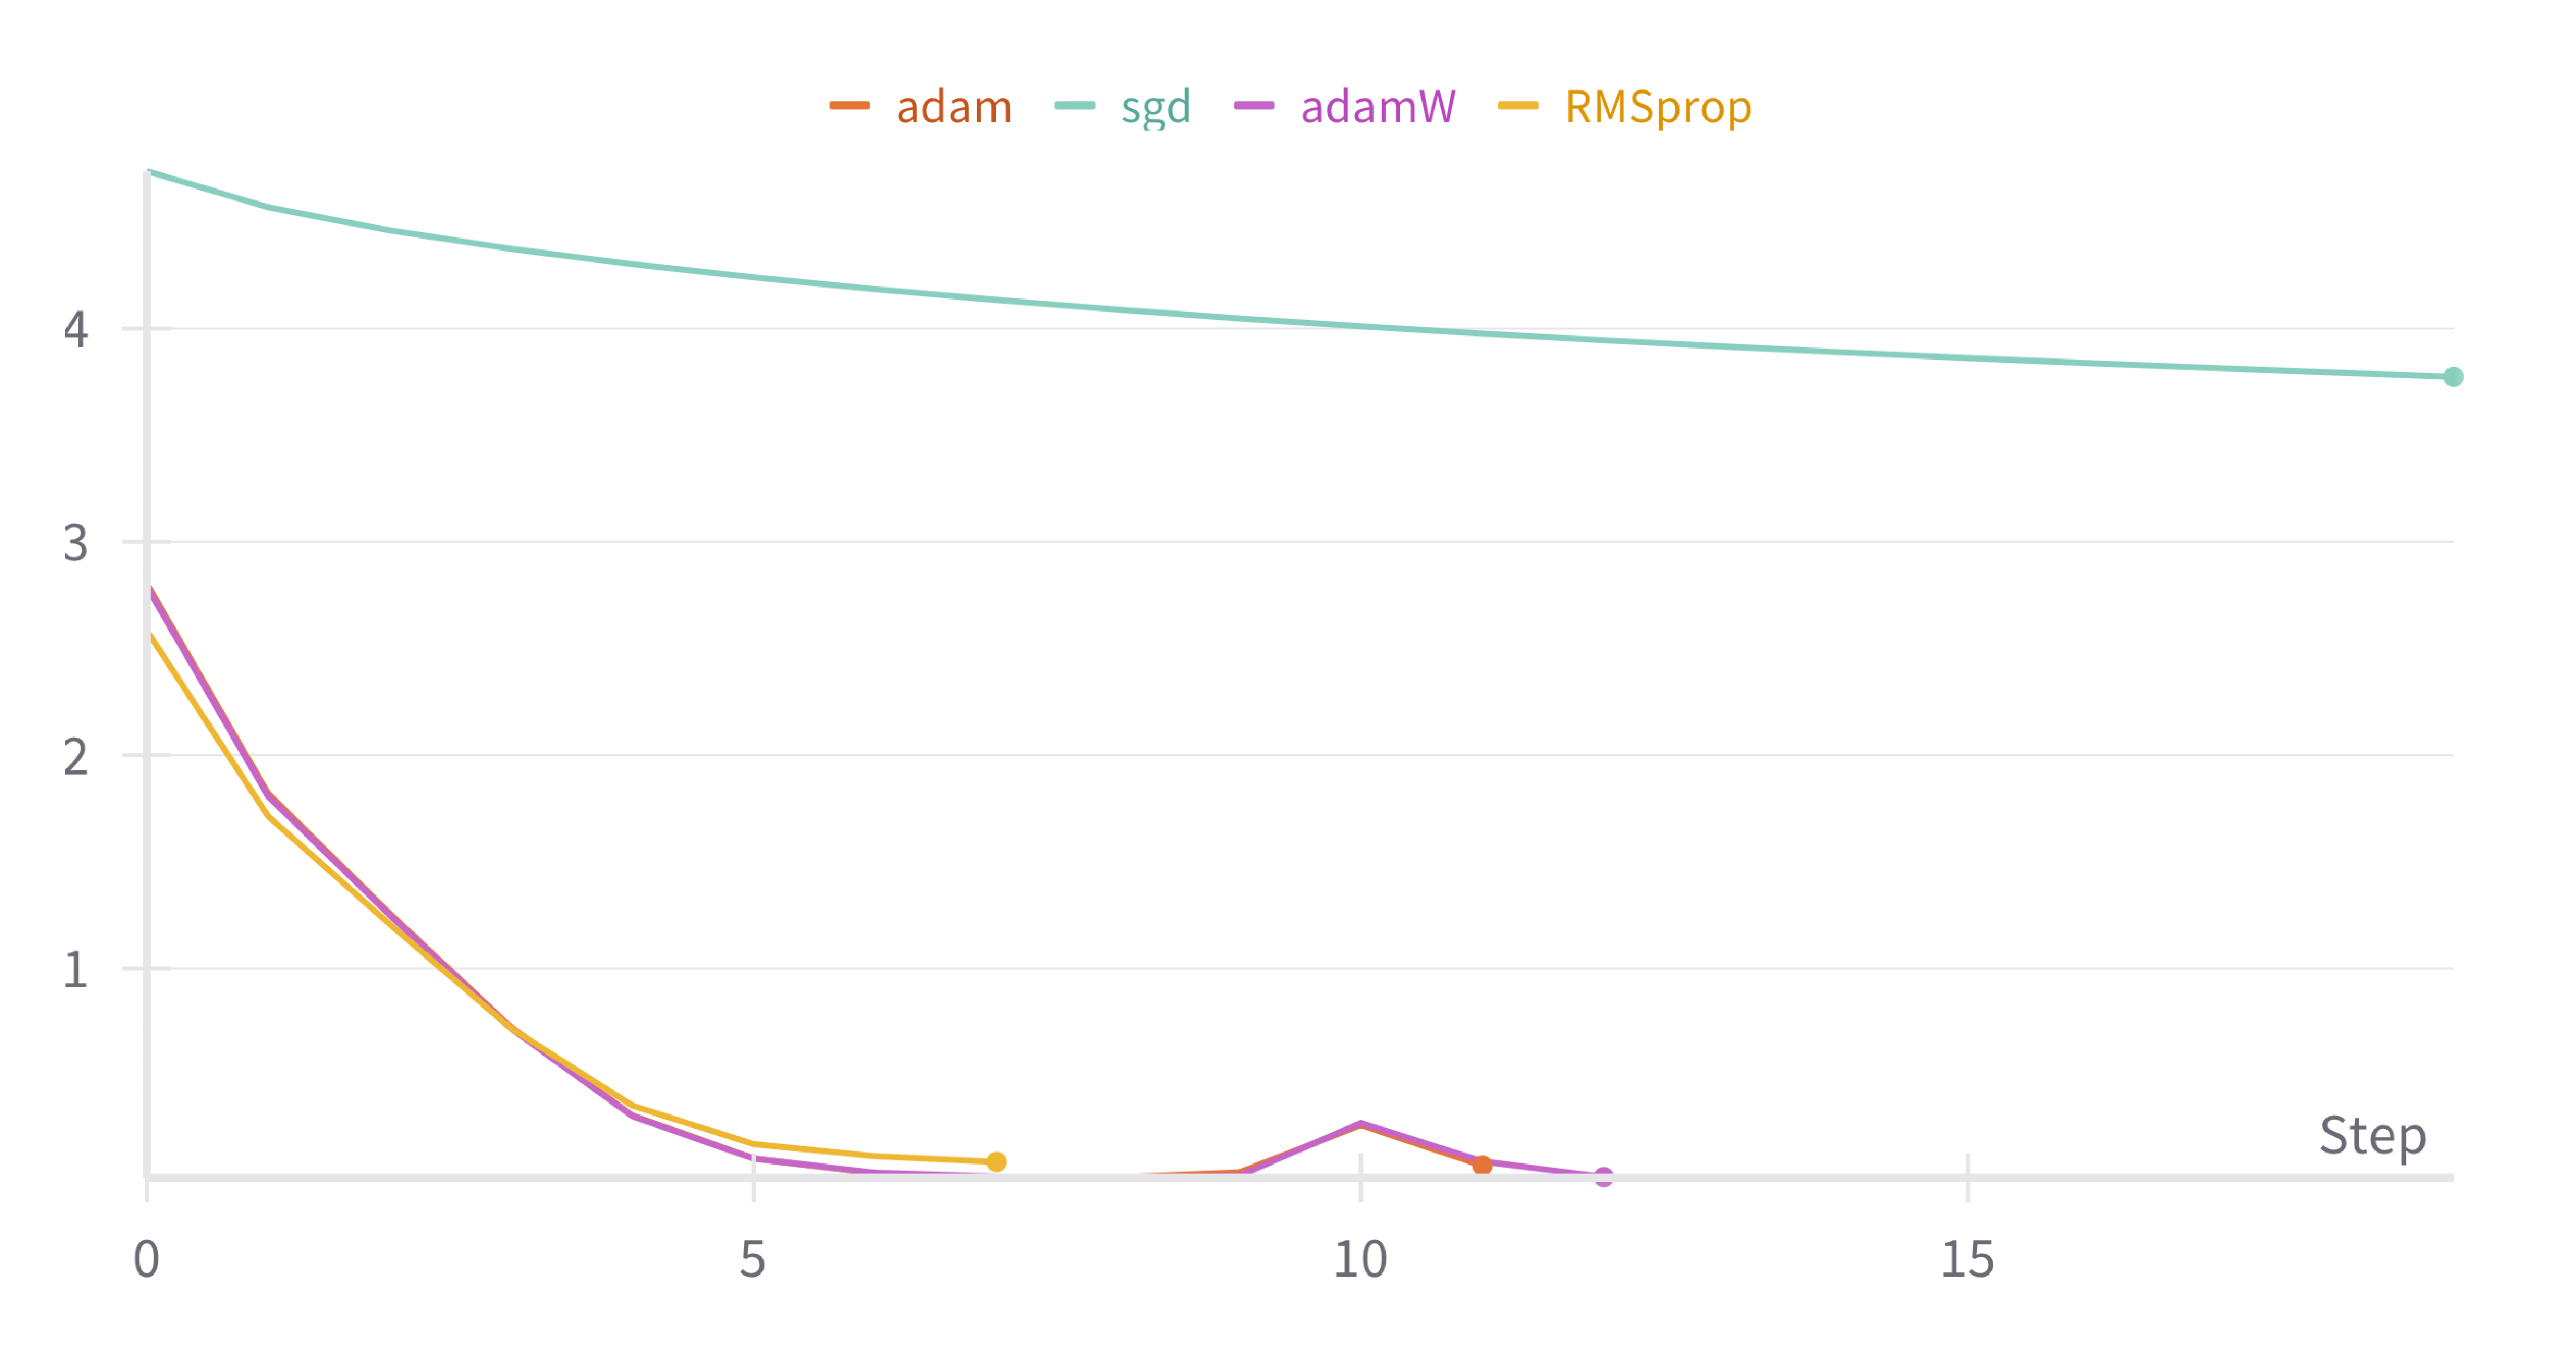
\includegraphics[width=\textwidth]{immages/5-fine tune/loss opt 1.pdf}
        \caption{Loss}
    \end{subfigure}
    \hfill
    \begin{subfigure}{0.45\textwidth}
        \centering
        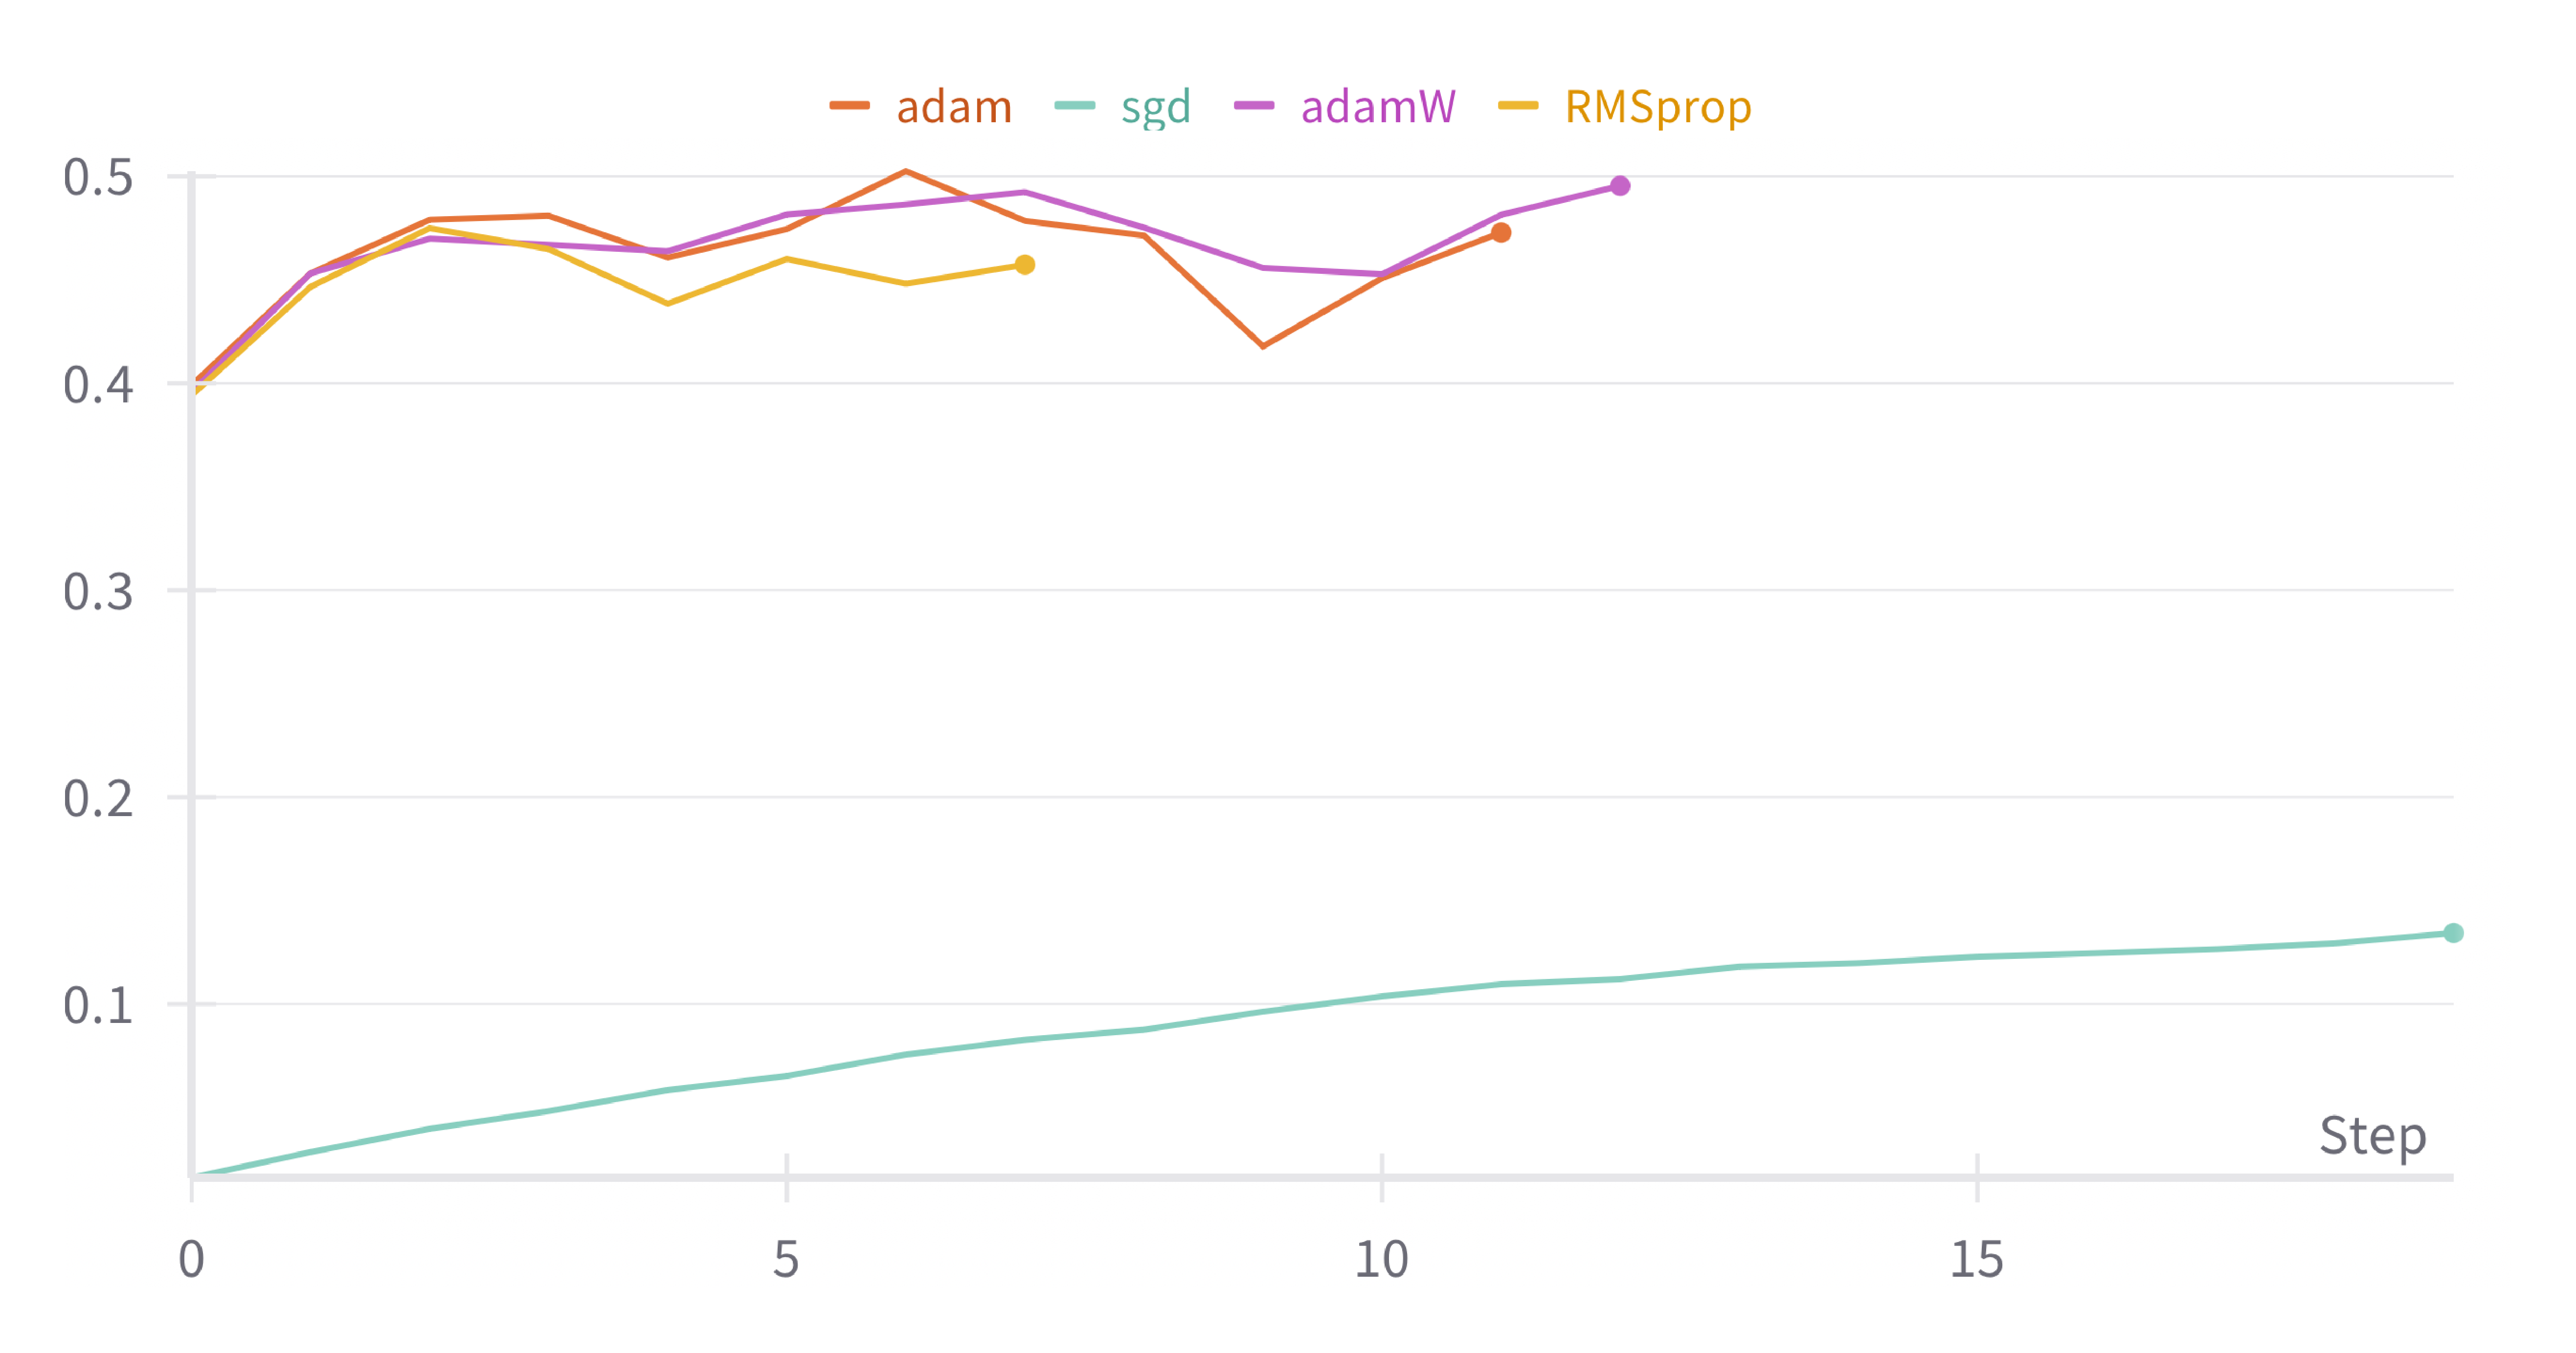
\includegraphics[width=\textwidth]{immages/5-fine tune/acc opt 1.pdf}
        \caption{Accuracy}
    \end{subfigure}
    \caption{Esperimento con diversi ottimizzatori e \texttt{lr=5e-4}}
    \label{fig:opt1}
\end{figure}

\myskip

Ho allora abbassato il learning rate a $10^{-5}$ e i risultati sono stati più soddisfacenti. Come si osserva dalla Figura \ref{fig:opt2} le prestazioni di SGD sono ancora di molto inferiori agli altri sia confrontando la loss sul training set che l'accuracy sul validation set. Gli altri 3 ottimizzatori sono invece confrontabili: quello che ha avuto risultati migliori è stato Adam classico. Questo sarà anche l'ottimizzatore utilizzato nelle fasi successive.

\begin{figure}[htbp]
    \centering
    \begin{subfigure}{0.45\textwidth}
        \centering
        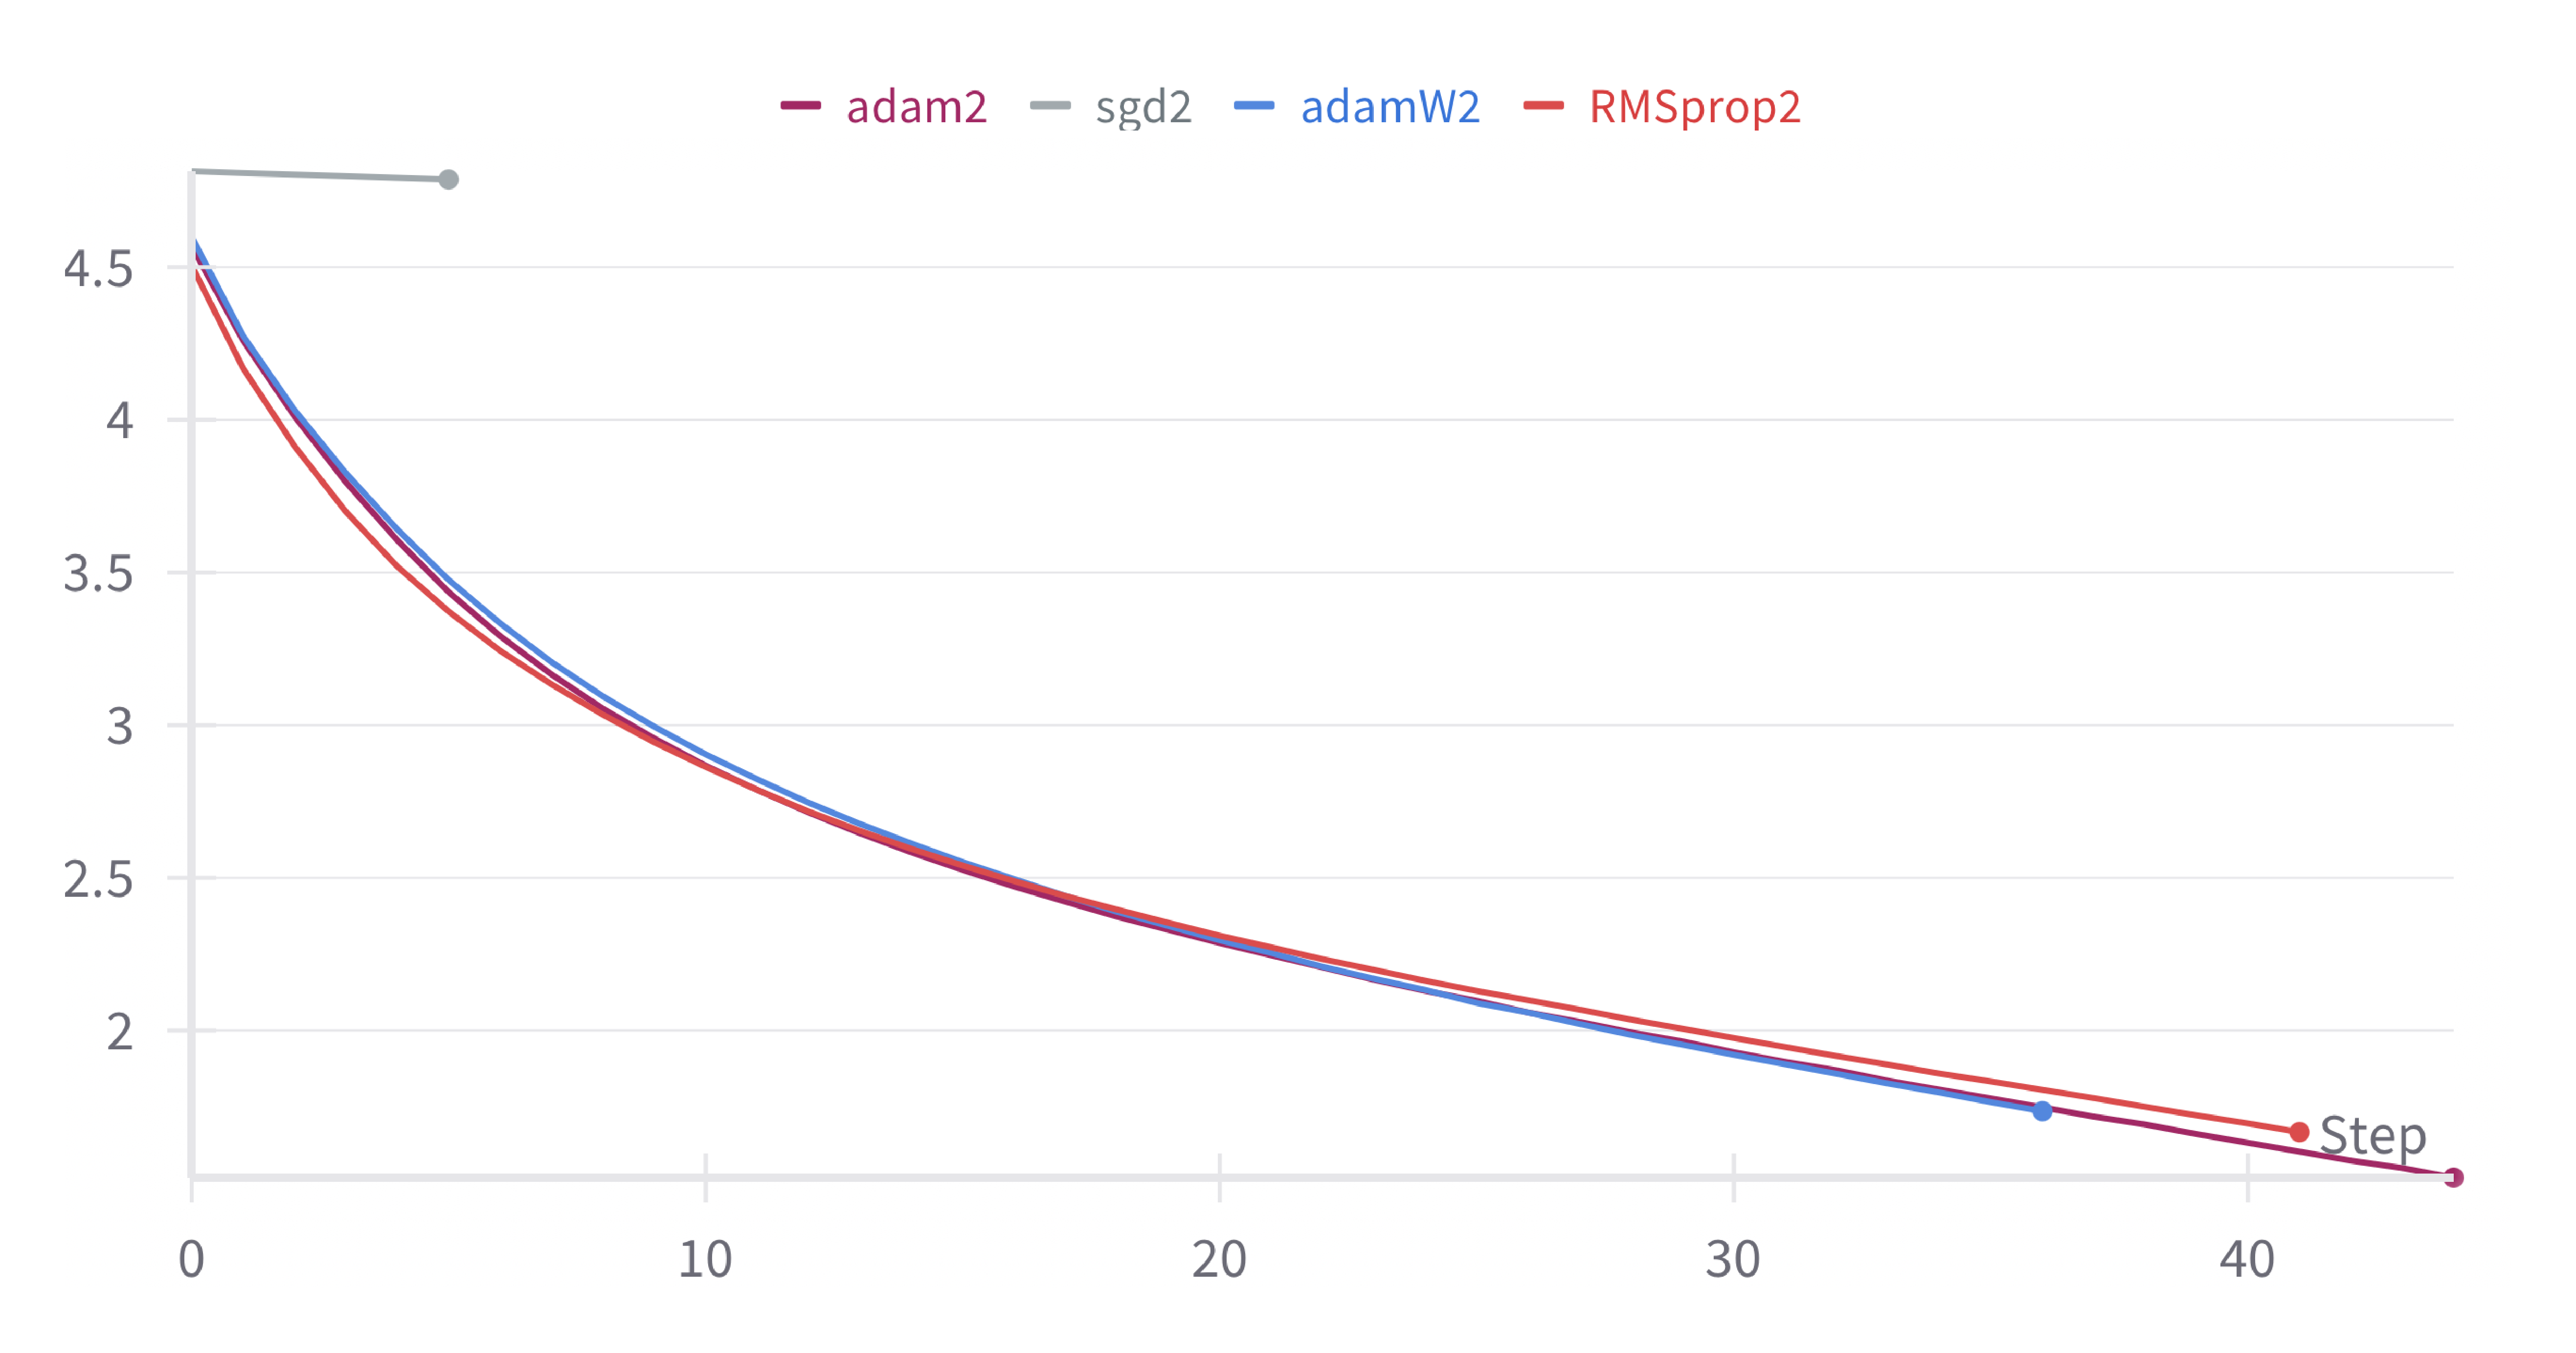
\includegraphics[width=\textwidth]{immages/5-fine tune/loss opt 2.pdf}
        \caption{Loss}
    \end{subfigure}
    \hfill
    \begin{subfigure}{0.45\textwidth}
        \centering
        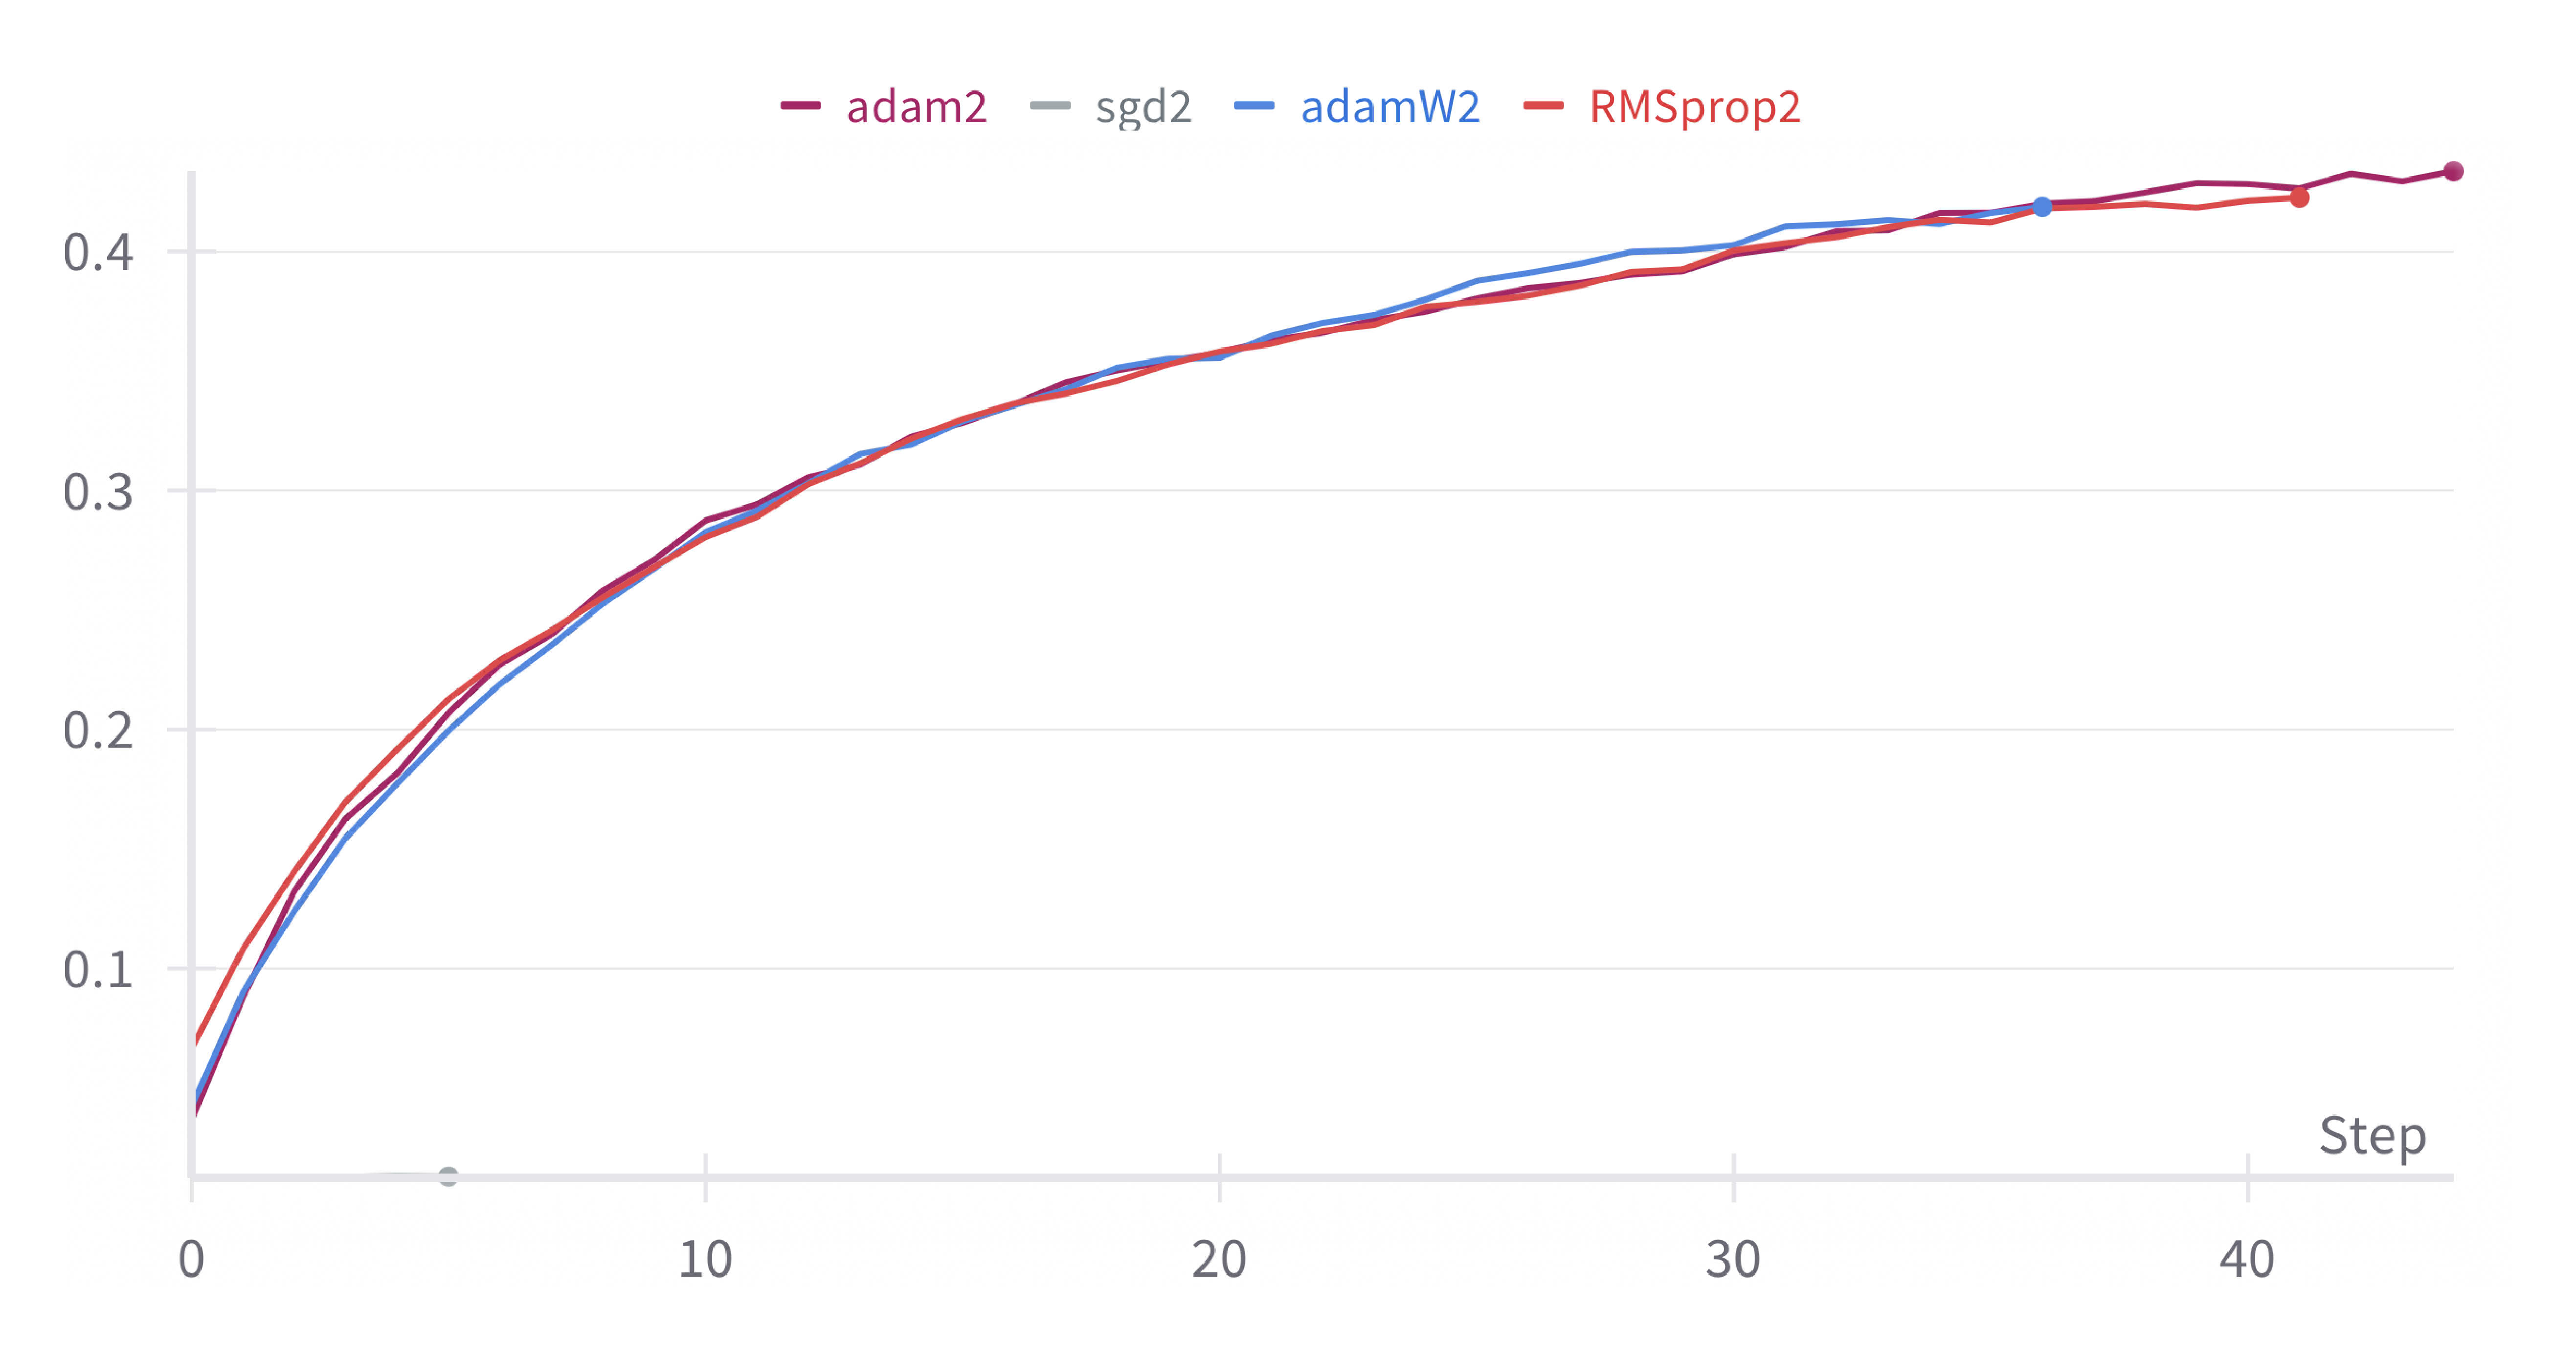
\includegraphics[width=\textwidth]{immages/5-fine tune/acc opt 2.pdf}
        \caption{Accuracy}
    \end{subfigure}
    \caption{Esperimento con diversi ottimizzatori e \texttt{lr=1e-5}}
    \label{fig:opt2}
\end{figure}

\myskip

Quello che rimarrebbe da fare è testare i vari algoritmi con learning rate a metà tra quelli testati. Questo però è fatto nella ricerca degli iperparametri nella sezione successiva.

%%%%%%%%%%%%%%%%%%%%%%%%%%%%%%%%%%%%%%%%%%%%%%%%%%%%
\section{Iperparametri}
\label{sec:iperparametri}
Cerchiamo di trovare i migliori iperparametri del modello. Gli iperparametri presi in considerazione sono:
\begin{itemize}
    \item Learning rate \\
        L'idea è quella di considerare un learning rate che possa andare da $10^{-2}$ fino a $10^{-6}$. Questa variabilità non è decisa in modo discreto, ma è lasciata allo sweeper di W\&B, che decide il valore campionandolo all'interno dell'intervallo.
    \item Batch size \\
        Come possibili valori ho considerato 32, 64, 128 e 256.
\end{itemize}

\myskip

\begin{figure}[htbp]
    \centering
    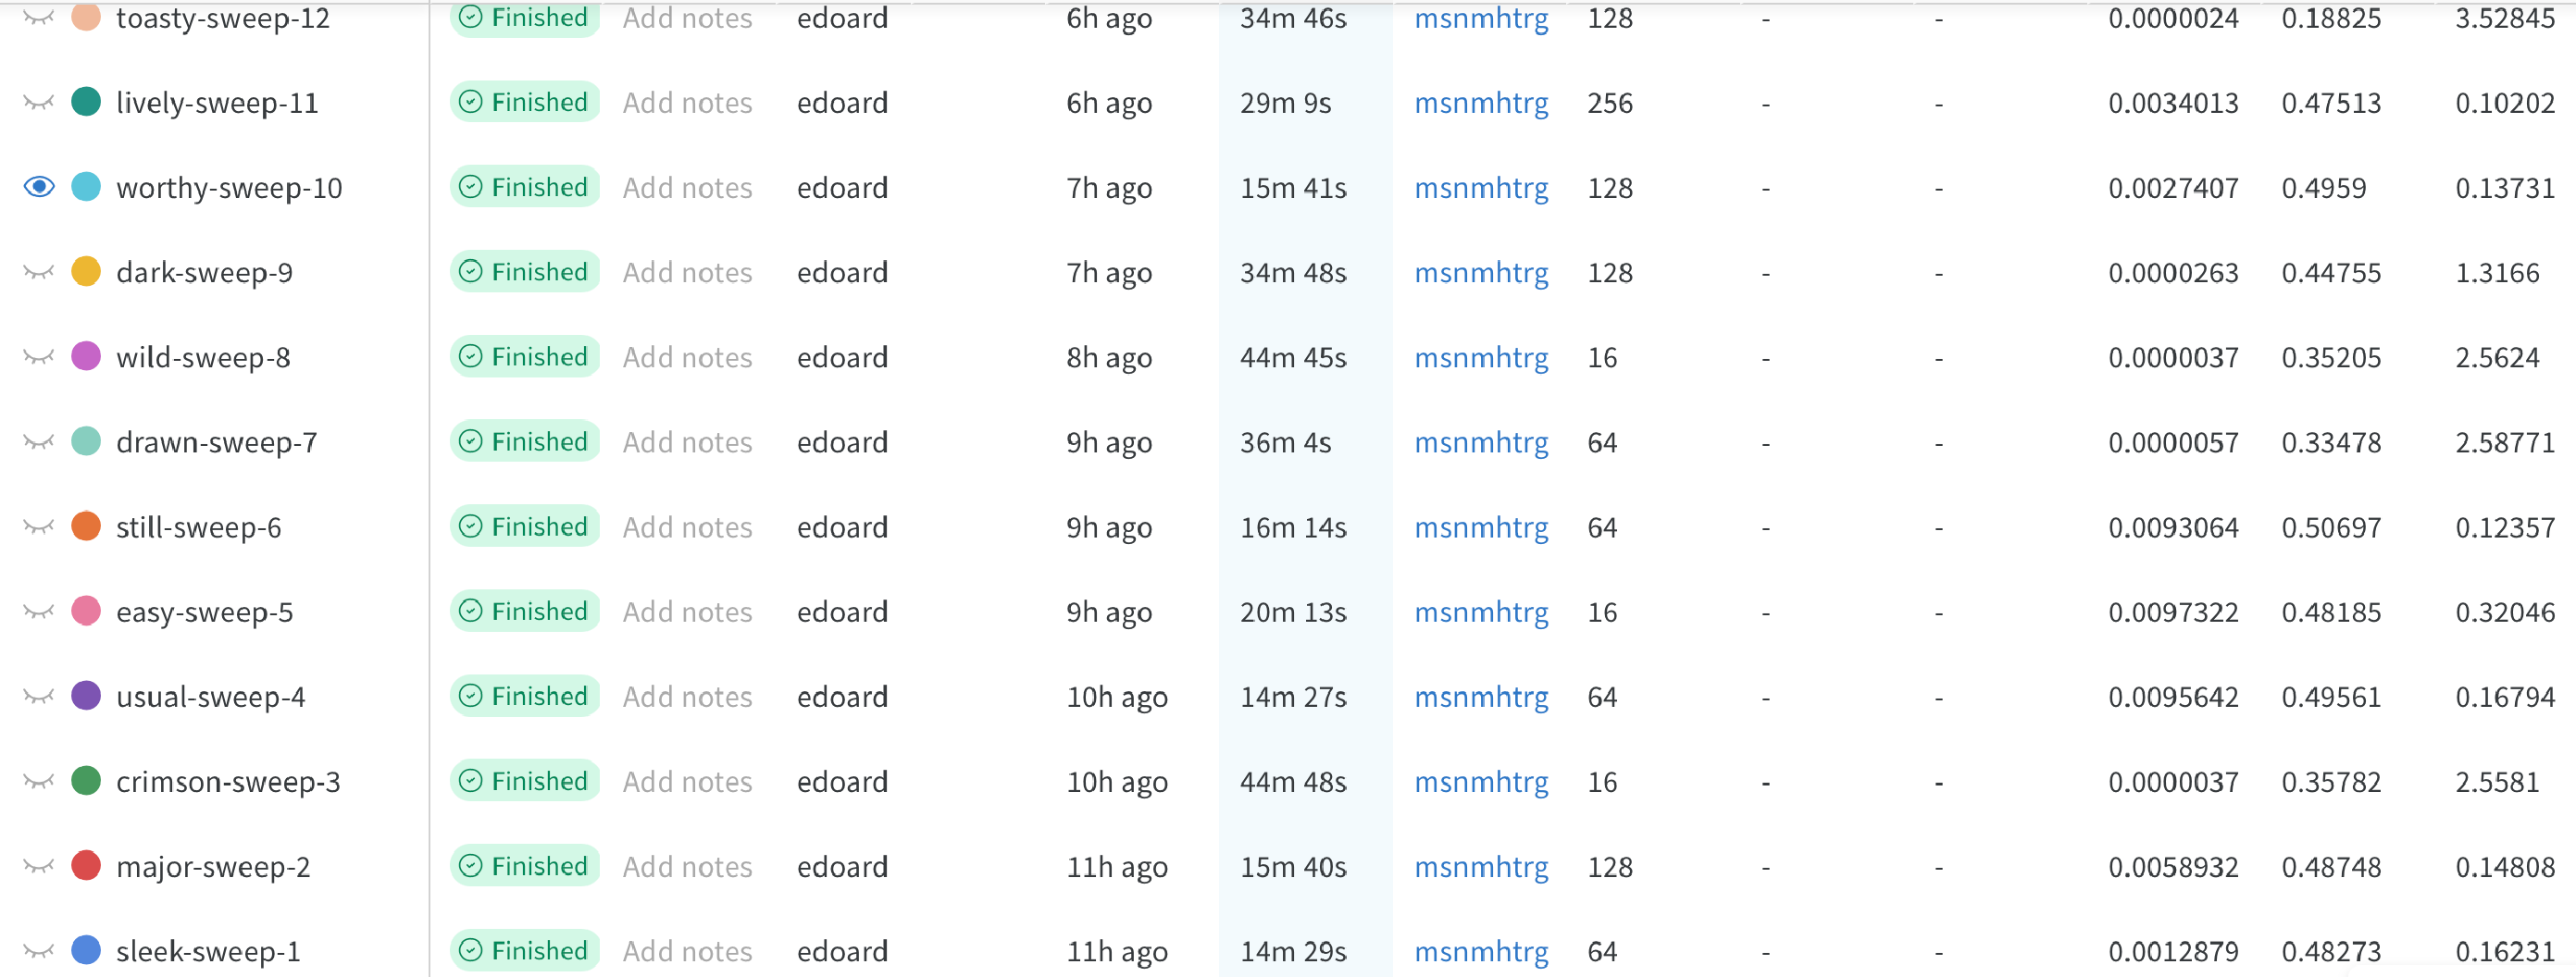
\includegraphics[width=0.9\textwidth]{immages/5-fine tune/esperimenti.pdf}
    \caption{Ricerca degli iperparametri}
    \label{fig:esperimenti}
\end{figure}

Come si vede dalla Figura \ref{fig:esperimenti} sono stati eseguiti 12 esperimenti.

Se osserviamo gli esperimenti che sono andati meglio (4, 6 e 10) in Figura \ref{fig:esperimentiok} possiamo osservare che il learning rate è dello stesso ordine di grandezza ($\mathcal{O}{(10^{-3})}$), mentre il batch size è 64 in due casi e 128 nell'altro. Nel prossimo paragrafo addestreremo il modello con learning rate e batch size dell'esperimento 6, il migliore registrato.

\begin{figure}[htbp]
    \centering
    \begin{subfigure}{0.45\textwidth}
        \centering
        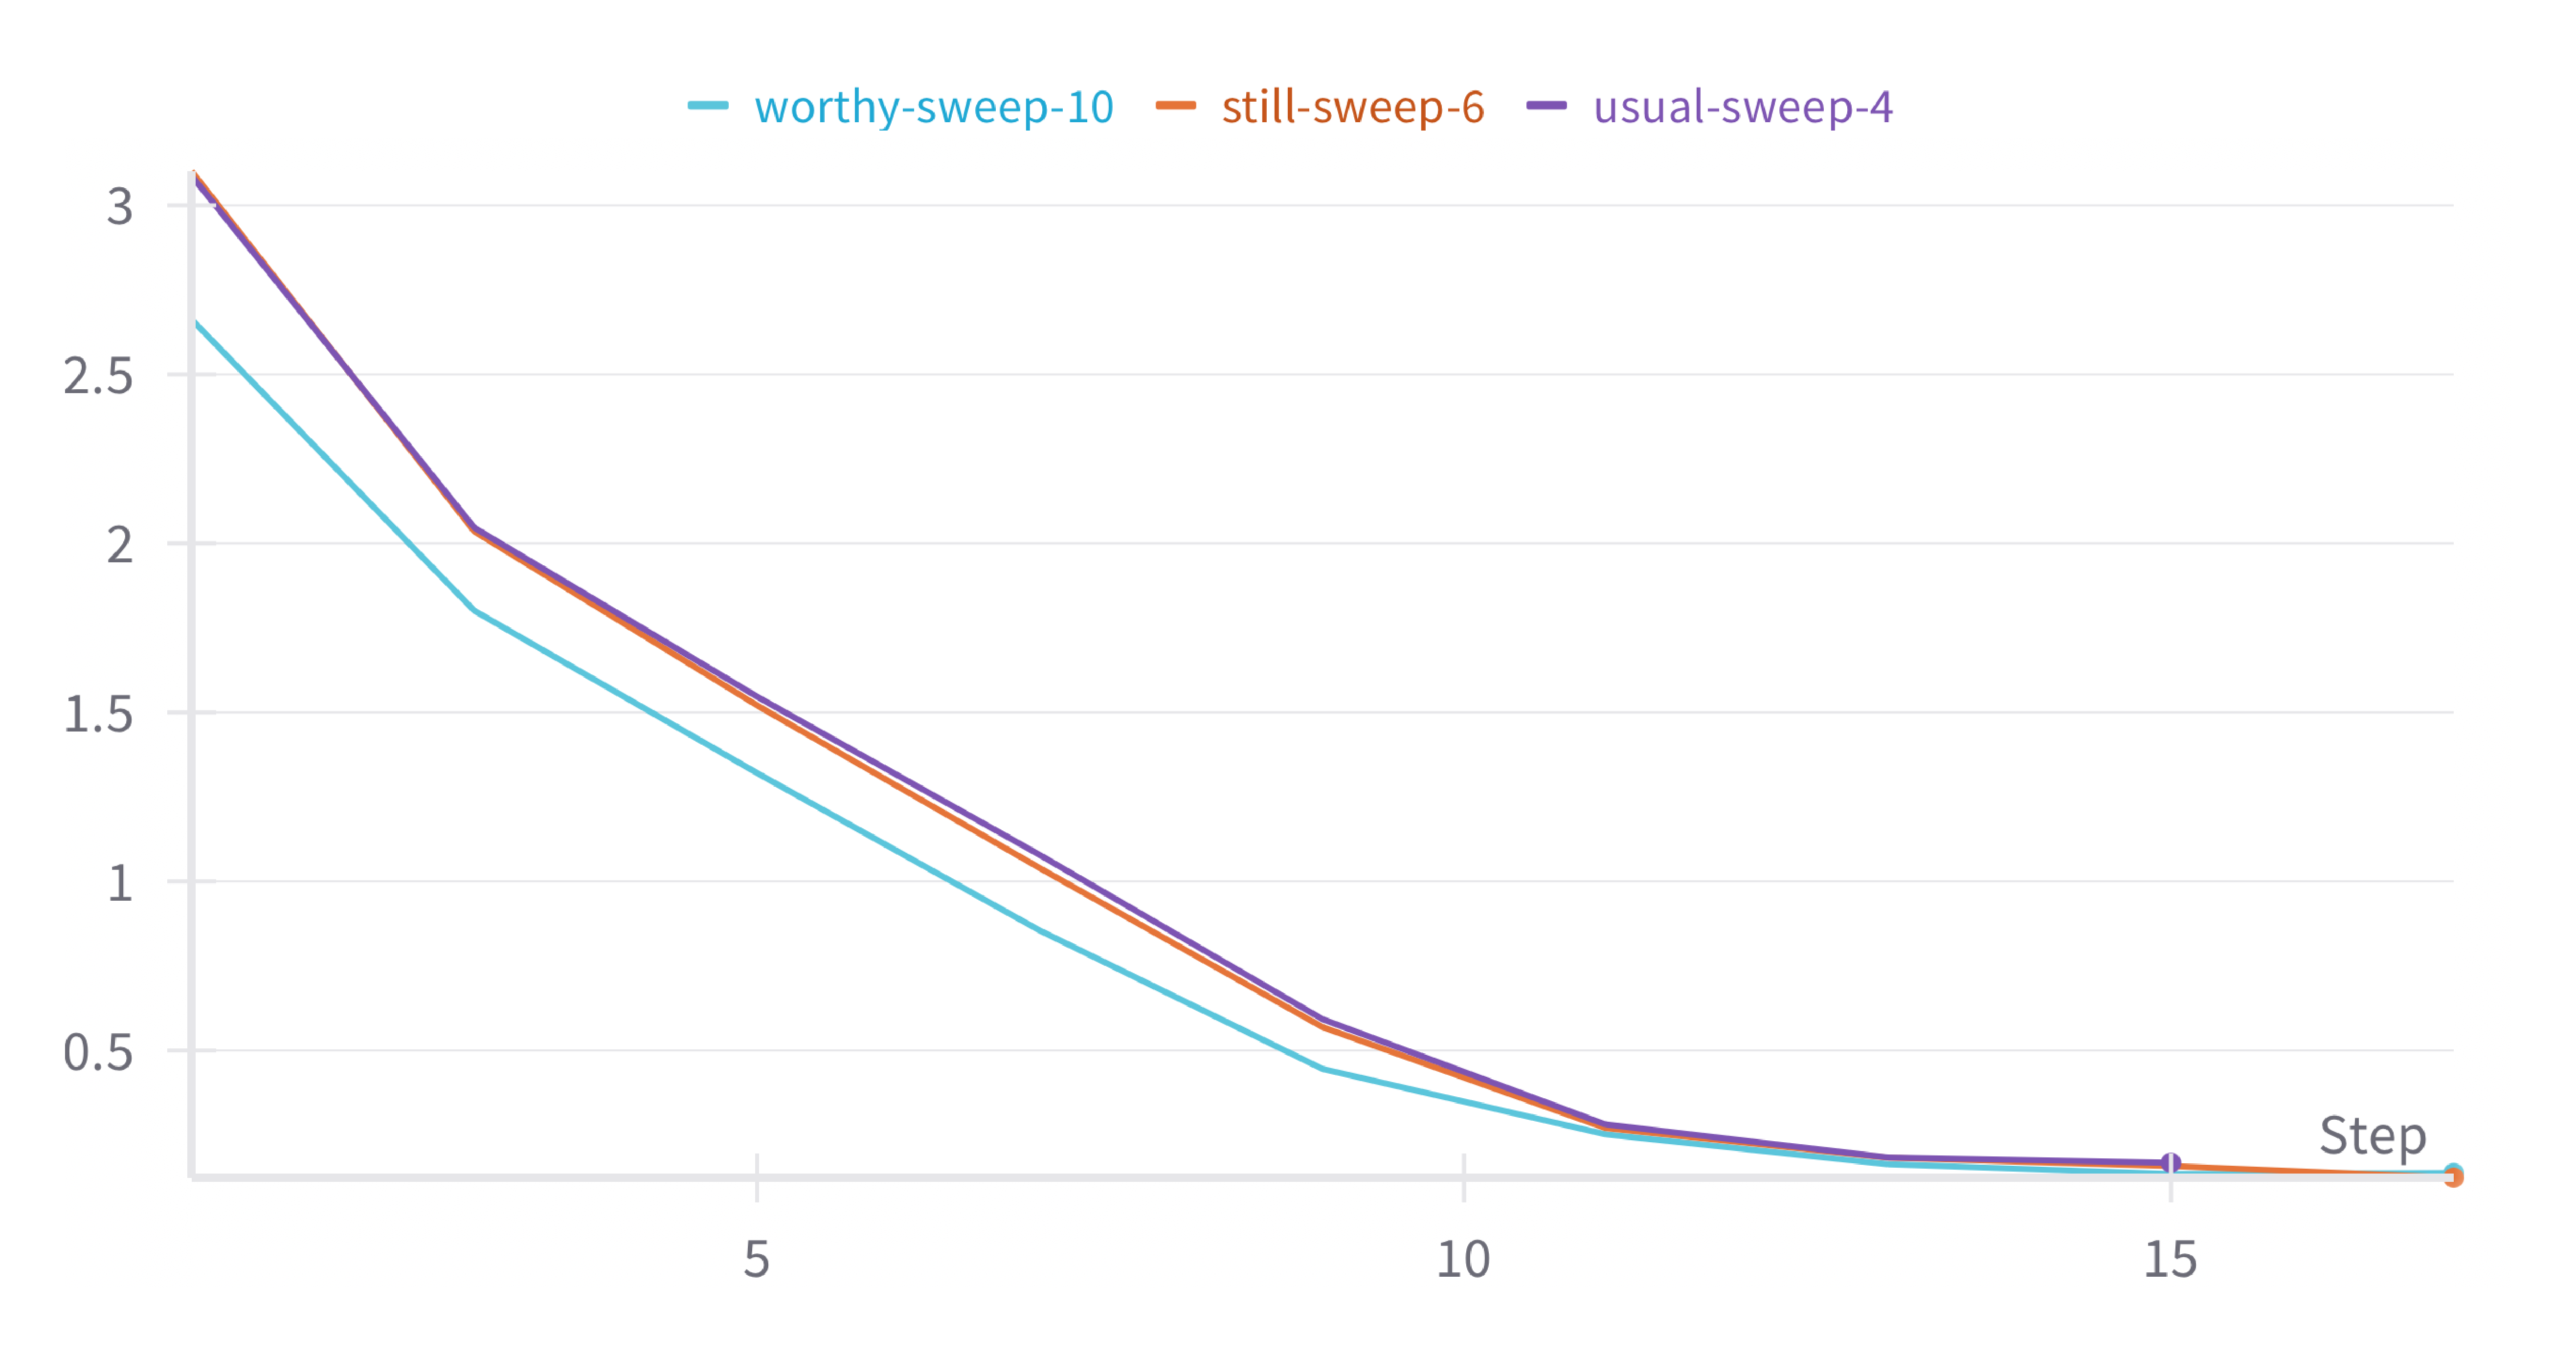
\includegraphics[width=\textwidth]{immages/5-fine tune/loss ok esperimenti.pdf}
        \caption{Loss}
    \end{subfigure}
    \hfill
    \begin{subfigure}{0.45\textwidth}
        \centering
        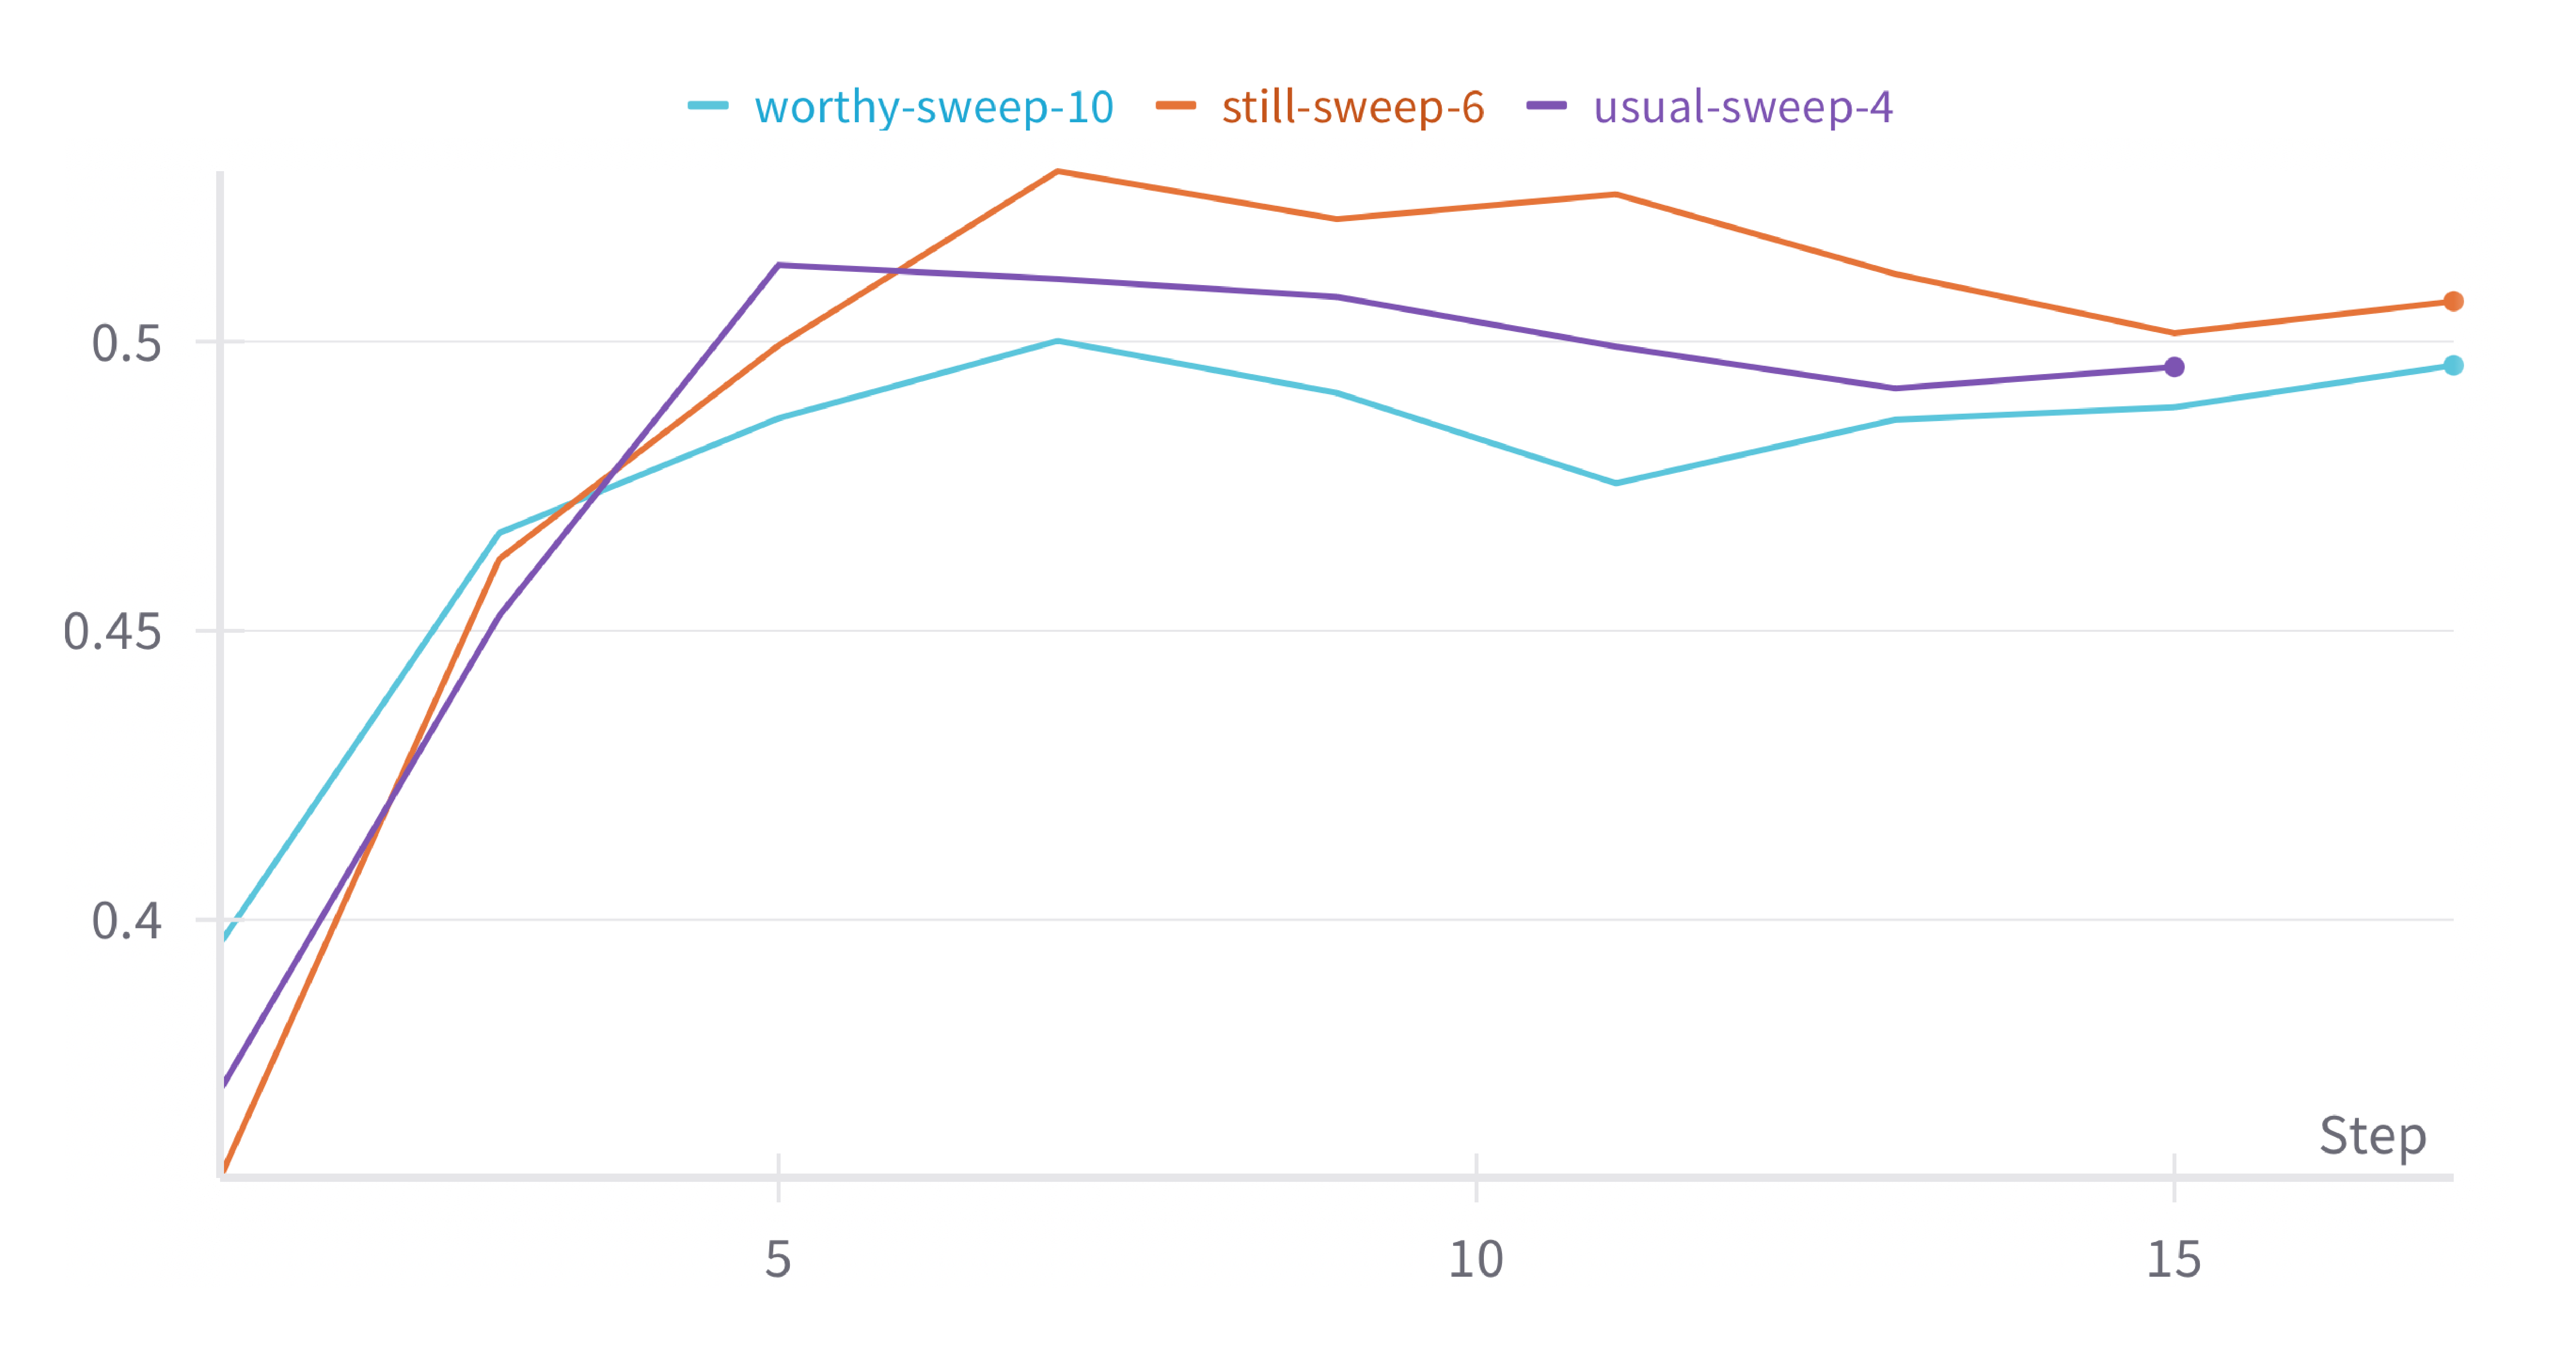
\includegraphics[width=\textwidth]{immages/5-fine tune/acc ok esperimenti.pdf}
        \caption{Accuracy}
    \end{subfigure}
    \caption{Ricerca degli iperparametri: esperimenti migliori.}
    \label{fig:esperimentiok}
\end{figure}

%%%%%%%%%%%%%%%%%%%%%%%%%%%%%%%%%%%%%%%%%%%%%%%%%%%%
\section{Dropout e generalizzazione}
Vediamo ora come il miglior modello che abbiamo ottenuto si comporta nell'addestramento e come generalizza sui dati mai visti del test set. Gli iperparametri utilizzati sono quelli ricavati alla Sezione \ref{sec:iperparametri}.

In Figura \ref{fig:dropout} si possono osservare le metriche ottenute durante l'addestramento: la loss sul train set e l'accuracy sul validation set. Possiamo notare come l'accuracy ottenuta usando il dropout durante l'addestramento sia la migliore riscontrata fino a questo momento.

L'accuracy ottenuta sul test set è stata invece di circa 0,51; questo risultato è verificabile solo eseguendo il codice. Ovviamente è normale che sul test set l'accuracy sia più bassa rispetto a quella sul validation set. Però il fatto che non sia comunque troppo inferiore ci fa capire che il modello generalizza abbastanza bene.

\begin{figure}[htbp]
    \centering
    \begin{subfigure}{0.45\textwidth}
        \centering
        \includegraphics[width=\textwidth]{immages/5-fine tune/loss dropout.pdf}
        \caption{Loss}
    \end{subfigure}
    \hfill
    \begin{subfigure}{0.45\textwidth}
        \centering
        \includegraphics[width=\textwidth]{immages/5-fine tune/acc dropout.pdf}
        \caption{Accuracy}
    \end{subfigure}
    \caption{Esperimento con dropout.}
    \label{fig:dropout}
\end{figure}